\documentclass{article}
\usepackage{graphicx}
\usepackage{amsmath, amssymb, amsthm}
\usepackage{csvsimple}
\usepackage{indentfirst}
\usepackage{caption}

\author{Elnur Gasanov : 163411}
\title{HW 5: Decision Trees}

\parindent=2mm

\begin{document}
\maketitle

\section{Constructing Decision Tree}

The code calculates Gain Ratio (GR) for all possible splits of attribute values. Since it is not stated strictly, we consider that attributes Age and Salary can be divided only into 3 or 4 group of values. Below the correspondence between age and salary groups and numbers are shown.

\begin{tabular}{|c|c|c|c|c|c|c|}
	\hline
	age & 21-25 & 26-30 & 31-35 & 36-40 & 41-45 & 46-50 \\
	\hline
	group & 0 & 1 & 2 & 3 & 4 & 5 \\
	\hline
\end{tabular}

\begin{tabular}{|c|c|c|c|c|c|c|}
	\hline
	salary & 26-30K & 31-35K & 36-40K & 41-45K & 46-50K & 66-70K \\
	\hline
	group & 1 & 2 & 3 & 4 & 5 & 6 \\
	\hline
\end{tabular}

At the root the largest GR (0.282) is attained when dividing salary into 3 groups ([1, 2], [3], [4, 5, 6]). Workers whose salary is in range [1, 2] have junior status, others who earns the amount of money from 3rd group are senior workers, that's why we further divide only the right branch.

In the right branch the largest GR (surprisingly, 0.588) is attained by dividing the age into 3 groups: [0, 1], [2, 3, 4], [5]. All workers whose age is in range [0, 1] have junior status. On the other hand, there is no data for ones whose age is in group 5. We "randomly" set the status to be "senior" for data in this group. Further we divide the middle branch.

The largest GR (0.207) in the middle branch is attained when dividing the salary into 3 groups:4, 5, 6. Then all leaves have specific value for status. 

The resulting decision tree is show on the figure~\ref{DT1}.

\begin{figure}
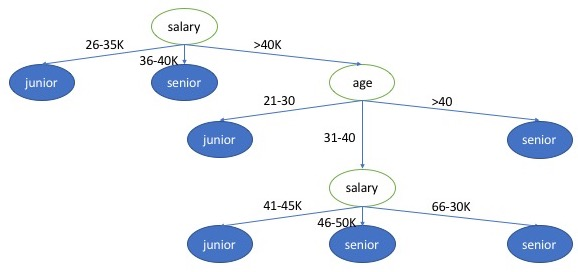
\includegraphics[width=\textwidth]{DT1}
\caption{Decision Tree with branching factor 3,4 for attributes Age and Salary}
\label{DT1}
\end{figure}

Now let us suppose that branching factor 2 for attributes Age and Salary is allowed. Then we get different decision tree.

At the root the largest GR (0.325) is attained by division of age into two groups of values ([0, 1, 2], [3, 4, 5]). All workers elder 36yo have status "senior".

In the left branch the largest GR (0.276) is attained by division of salary into two groups of values ([1, 2, 3, 4, 5], [6]). All workers in this branch earning 66-70K (group 6) have status "senior".

Then the best GR is got when dividing salary again into two groups: [1, 2, 3, 4], [5]. Then all leaves have the specific value of status. 


The resulting decision tree is show on the figure~\ref{DT2}.

\begin{figure}
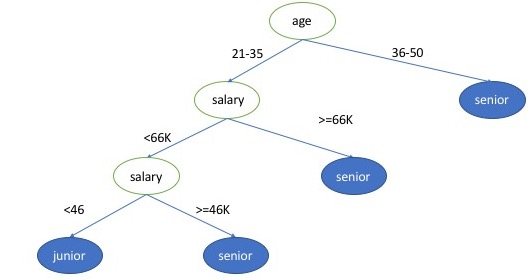
\includegraphics[width=\textwidth]{DT2}
\caption{Decision Tree with branching factor 2,3,4 for attributes Age and Salary}
\label{DT2}
\end{figure}

\section{Applying DT}

The first DT gives status "junior" whilst the second one determines the object as senior worker.

\section{Naive Bayes}

$p(systems | junior) =  0.2305, \ p(systems | senior) = 0.154, \ p(26..30 | junior) = 0.4336, \ p(26..30 | senior) = 0, \ p(46-50K| junior) = 0.2035, \ p(46-50K|senior) = 0.19$. Since $p(26..30 | senior) = 0$ and there are no other zero probabilities, naive Bayes will give status "junior" for an object.

\end{document}